%%
%% Author: thompson
%% 26.10.17
%%

% Preamble
\documentclass[11pt]{article}

% Packages
\usepackage{a4wide}
\usepackage[utf8]{inputenc}
\usepackage[ngerman]{babel}
\usepackage{scrextend}      % Intending
\usepackage{graphicx}

% Document
\begin{document}

\section{ISO-OSI Referenzmodel}

    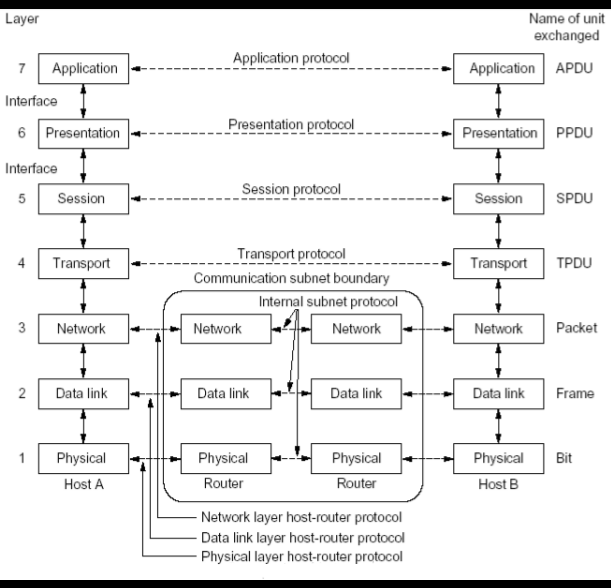
\includegraphics[width=\textwidth]{ISO_OSIReferenceModel.png}

    Das ISO-OSI Referenzmodell besteht aus verschiedenen Anwendungsschichten:
    \begin{enumerate}
        \item Physical Layer\\
        Dieser Layer beschreibt die fundamentale Netzwerkkommunikation. Datentransfer via
        physischem Layer sind reine Bitstreams.
        \item Data Link Layer\\
        Der Datenlink nutzt Frames zur Übertragung von Datensätzen. Frames bestehen aus einer gewissen Anzahl
        an Bit-Blöcken und einer Prüfsumme, welche die korrekte Datenflussübertragung gewährleistet.
        Fehlerbehafte Frames können anhand dieser Summe erkannt werden und der DLL kann das jeweilige Paket verwerfen
        oder sogar korrigieren.
        Im Falle des Verwerfens ist es allerdings nicht vorgesehen das jeweilige Frame neu anzufordern.

        Mithilfe der 'Data Flow Control' kann man die Dynamik der Frameübertragung steuern, etwa wie schnell
        Blöcke verschickt werden.

        Genutzte Hardware:
        \begin{addmargin}[1em]{1em} % Left & right
            Bridge \& Switch: Arbeiten via Media Access Control(Mac) oder Logical Link Control(LLC).\\
            Die MAC-Bridge schützt gegen Kollisionen via Aufteilung des Netzes in verschiedene Kollisionsdomänen, d.H.
            ein Paket geht nur in das Netz, in welchem sich der tatsächliche Empfänger befindet.\\
            Die LLC-Bridge dient der Koppelung zweier Teilnetze mithilfe verschiedener Zugriffsverfahren, wie
            Token-Passing (Tokens werden zwischen Sendern gewechselt und dementsprechend startet Datenverkehr) oder
            Carrier Sense Multiple Access/Collision Detection (CSMA/CD; Typischer Router mit x-Medien).\\
        \end{addmargin}

        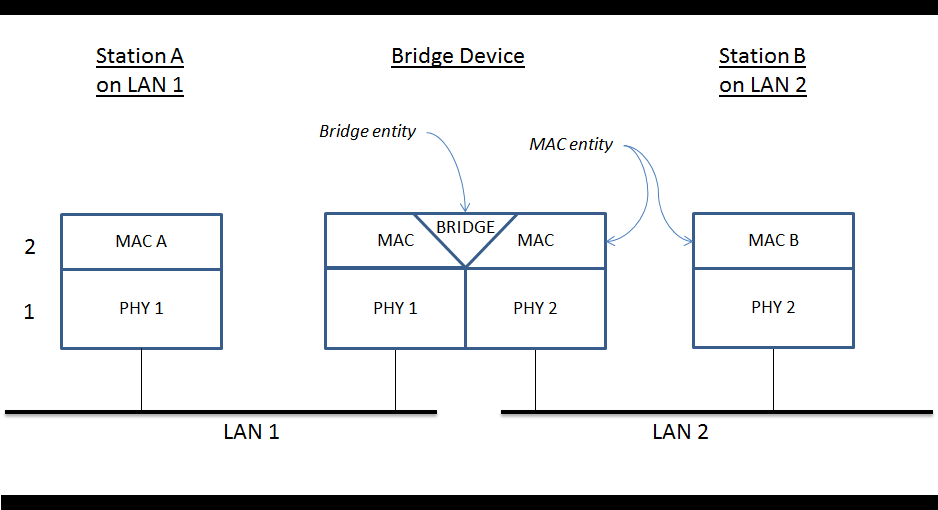
\includegraphics[width=\textwidth]{Network_Bridging.png}
        \footnote[1\small \emph{Schemata of Bridge/Switch inside a Network}]{By Crvincenzi - MS Powerpoint, CC BY-SA 3.0, https://commons.wikimedia.org/w/index.php?curid=25610536}

        Protokolle: HDLC, SDLC, DDCMP, Shortest Path Bridging
        Normen: IEEE, FDDI

        \item Network Layer
        \item Transport Layer
        \item Session Layer
        \item Presentation Layer
        \item Application Layer
    \end{enumerate}

\end{document}